% One Trotter step of TEBD: the nearest-neighbour terms of the Hamiltonian do
% not commute, so the step is split into the odd bonds and then the even ones,
% and each half is a row of two-site gates that do commute among themselves.
%
% The tensors are plain arrays rather than the canonical triangles, because a
% Trotter step does not care which way the gauge runs -- it is applied to the
% physical indices and the gauge is restored afterwards, by the truncation that
% is not drawn here.
%
% No gate has legs of its own. The physical indices run the whole way down and
% a gate is laid on the ones it acts on; a tensor is drawn over an index, so it
% interrupts them, which is what applying it means. Read downward: the state,
% the odd bonds, the even bonds, and the indices that come out are the same
% indices that went in.
\documentclass[border=4pt]{standalone}
\usepackage{amsmath,amssymb}
\usepackage{tikz-tensors}
\begin{document}
\begin{tikzpicture}[x=1.25cm]
  \tnchain{S}{(0,0)}{(5,0)}{coef/$A$/c, coef/$A$/c, coef/$A$/c,
                            coef/$A$/c, coef/$A$/c, coef/$A$/c}
  \foreach \i [evaluate=\i as \j using int(\i+1)] in {1,...,5}{
    \tnbond[disc]{(S\i) -- (S\j)}%
  }
  \tnbond[disc]{([xshift=-5mm]S1.west) -- (S1)}
  \tnbond[disc]{([xshift=5mm]S6.east) -- (S6)}

  % the physical indices, the whole way down
  \tnlegs{34mm}{S1-leg,S2-leg,S3-leg,S4-leg,S5-leg,S6-leg}

  % the odd bonds, then the even ones
  \tngate{Oa}{$U$}{S1-leg,S2-leg}{9mm}
  \tngate{Ob}{$U$}{S3-leg,S4-leg}{9mm}
  \tngate{Oc}{$U$}{S5-leg,S6-leg}{9mm}
  \tngate{Ea}{$U$}{S2-leg,S3-leg}{22mm}
  \tngate{Eb}{$U$}{S4-leg,S5-leg}{22mm}

  \foreach \i in {1,...,6}{ \tnput[below]{S\i-leg-tip}{$n_{\i}$}}
\end{tikzpicture}
\end{document}
